
\documentclass{article}

\usepackage{fancyhdr} % Required for custom headers
\usepackage{lastpage} % Required to determine the last page for the footer
\usepackage{extramarks} % Required for headers and footers
\usepackage[usenames,dvipsnames]{color} % Required for custom colors
\usepackage{graphicx} % Required to insert images
\usepackage{listings} % Required for insertion of code
\usepackage{courier} % Required for the courier font
\usepackage{lipsum} % Used for inserting dummy 'Lorem ipsum' text into the template
\usepackage{caption}
\usepackage{subcaption}

\graphicspath{ {../../../datasets/images/chapter_02/} }

% Margins
\topmargin=-0.45in
\evensidemargin=0in
\oddsidemargin=0in
\textwidth=6.5in
\textheight=9.0in
\headsep=0.25in

\linespread{1.1} % Line spacing

% Set up the header and footer
\pagestyle{fancy}
\lhead{\hmwkAuthorName} % Top left header
\chead{\hmwkClass\ (\hmwkClassInstructor\ \hmwkClassTime): \hmwkTitle} % Top center head
\rhead{\firstxmark} % Top right header
\lfoot{\lastxmark} % Bottom left footer
\cfoot{} % Bottom center footer
\rfoot{Page\ \thepage\ of\ \protect\pageref{LastPage}} % Bottom right footer
\renewcommand\headrulewidth{0.4pt} % Size of the header rule
\renewcommand\footrulewidth{0.4pt} % Size of the footer rule

\setlength\parindent{0pt} % Removes all indentation from paragraphs

%----------------------------------------------------------------------------------------
%	CODE INCLUSION CONFIGURATION
%----------------------------------------------------------------------------------------

\definecolor{MyDarkGreen}{rgb}{0.0,0.4,0.0} 
\lstloadlanguages{Matlab}
\lstset{language=Matlab,
        frame=single,
        basicstyle=\small\ttfamily,
        keywordstyle=[1]\color{Blue}\bf,
        keywordstyle=[2]\color{Purple},
        keywordstyle=[3]\color{Blue}\underbar,
        identifierstyle=,
        commentstyle=\usefont{T1}{pcr}{m}{sl}\color{MyDarkGreen}\small, 
        stringstyle=\color{Purple},
        showstringspaces=false,
        tabsize=5, 
        morekeywords={rand},
        morekeywords=[2]{on, off, interp},
        morekeywords=[3]{test},
        morecomment=[l][\color{Blue}]{...},
        numbers=left,
        firstnumber=1,
        numberstyle=\tiny\color{Blue},
        stepnumber=5
}

% Creates a new command to include a perl script, the first parameter is the filename of the script (without .pl), the second parameter is the caption
\newcommand{\matlabscript}[2]{
\begin{itemize}
\item[]\lstinputlisting[caption=#2,label=#1]{#1.m}
\end{itemize}
}

%----------------------------------------------------------------------------------------
%	DOCUMENT STRUCTURE COMMANDS
%	Skip this unless you know what you're doing
%----------------------------------------------------------------------------------------

% Header and footer for when a page split occurs within a problem environment
\newcommand{\enterProblemHeader}[1]{
\nobreak\extramarks{#1}{#1 continued on next page\ldots}\nobreak
\nobreak\extramarks{#1 (continued)}{#1 continued on next page\ldots}\nobreak
}

% Header and footer for when a page split occurs between problem environments
\newcommand{\exitProblemHeader}[1]{
\nobreak\extramarks{#1 (continued)}{#1 continued on next page\ldots}\nobreak
\nobreak\extramarks{#1}{}\nobreak
}

\setcounter{secnumdepth}{0} % Removes default section numbers
\newcounter{homeworkProblemCounter} % Creates a counter to keep track of the number of problems

\newcommand{\homeworkProblemName}{}
\newenvironment{homeworkProblem}[1][Problem \arabic{homeworkProblemCounter}]{ % Makes a new environment called homeworkProblem which takes 1 argument (custom name) but the default is "Problem #"
\stepcounter{homeworkProblemCounter} % Increase counter for number of problems
\renewcommand{\homeworkProblemName}{#1} % Assign \homeworkProblemName the name of the problem
\section{\homeworkProblemName} % Make a section in the document with the custom problem count
\enterProblemHeader{\homeworkProblemName} % Header and footer within the environment
}{
\exitProblemHeader{\homeworkProblemName} % Header and footer after the environment
}

\newcommand{\problemAnswer}[1]{ % Defines the problem answer command with the content as the only argument
\noindent\framebox[\columnwidth][c]{\begin{minipage}{0.98\columnwidth}#1\end{minipage}} % Makes the box around the problem answer and puts the content inside
}

\newcommand{\homeworkSectionName}{}
\newenvironment{homeworkSection}[1]{ % New environment for sections within homework problems, takes 1 argument - the name of the section
\renewcommand{\homeworkSectionName}{#1} % Assign \homeworkSectionName to the name of the section from the environment argument
\subsection{\homeworkSectionName} % Make a subsection with the custom name of the subsection
\enterProblemHeader{\homeworkProblemName\ [\homeworkSectionName]} % Header and footer within the environment
}{
\enterProblemHeader{\homeworkProblemName} % Header and footer after the environment
}

%----------------------------------------------------------------------------------------
%	NAME AND CLASS SECTION
%----------------------------------------------------------------------------------------

\newcommand{\hmwkTitle}{Assignment\ \#5}
\newcommand{\hmwkDueDate}{Monday,\ September\ 11,\ 2017}
\newcommand{\hmwkClass}{IMAGE\ PROCESSING} % Course/class
\newcommand{\hmwkClassTime}{14:00pm} % Class/lecture time
\newcommand{\hmwkClassInstructor}{gslee} % Teacher/lecturer
\newcommand{\hmwkAuthorName}{Tien Anh Nguyen} % Your name

%----------------------------------------------------------------------------------------
%	TITLE PAGE
%----------------------------------------------------------------------------------------

\title{
\vspace{2in}
\textmd{\textbf{\hmwkClass:\ \hmwkTitle}}\\
\normalsize\vspace{0.1in}\small{Due\ on\ \hmwkDueDate}\\
\vspace{0.1in}\large{\textit{\hmwkClassInstructor\ \hmwkClassTime}}
\vspace{3in}
}

\author{\textbf{\hmwkAuthorName}}
\date{} % Insert date here if you want it to appear below your name

%----------------------------------------------------------------------------------------

\begin{document}

\maketitle

%----------------------------------------------------------------------------------------
%	TABLE OF CONTENTS
%----------------------------------------------------------------------------------------

%\setcounter{tocdepth}{1} % Uncomment this line if you don't want subsections listed in the ToC

\newpage
\tableofcontents
\newpage

%----------------------------------------------------------------------------------------
%	PROBLEM 1
%----------------------------------------------------------------------------------------

% To have just one problem per page, simply put a \clearpage after each problem

\begin{homeworkProblem}
\maketitle
\subsection{Dilation}
\matlabscript{mfiles/exercise_dilation}{Dilation}


\newpage

\textbf{IM2 = imdilate(IM,SE)} dilates the grayscale, binary, or packed binary image IM,\
returning the dilated image, IM2. The argument SE is a structuring element object,\
or array of structuring element objects, returned by the \textbf{strel} or \textbf{offsetstrel} function.

\begin{figure}[h]
\centering
    \begin{subfigure}[t]{0.3\textwidth}
        \centering
        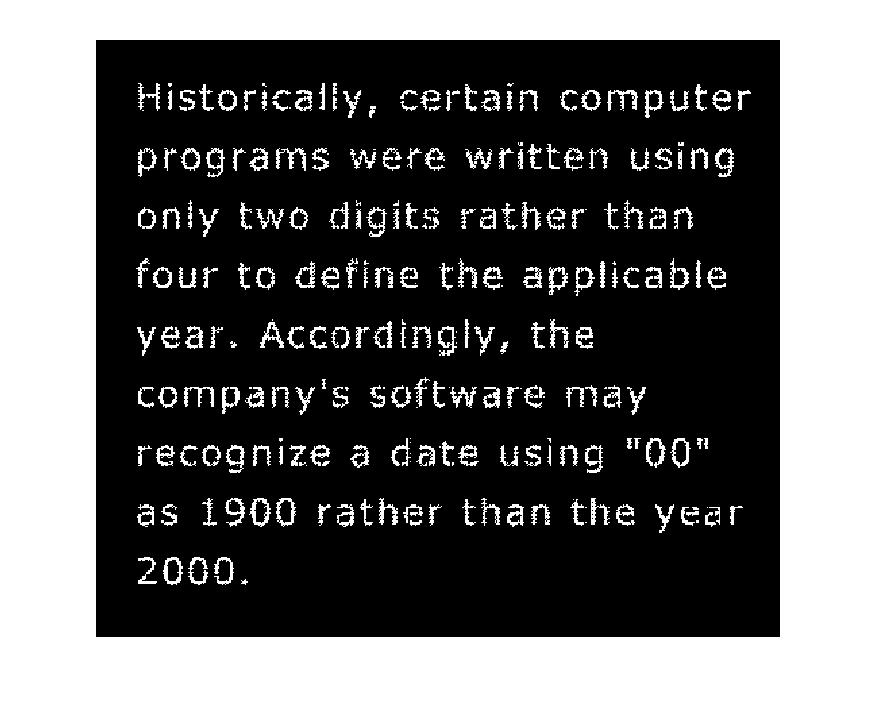
\includegraphics[height=1.2in]{figures/exercise_dilation_01.jpg}
        \caption{Original Image}
    \end{subfigure}%
    \begin{subfigure}[t]{0.3\textwidth}
        \centering
        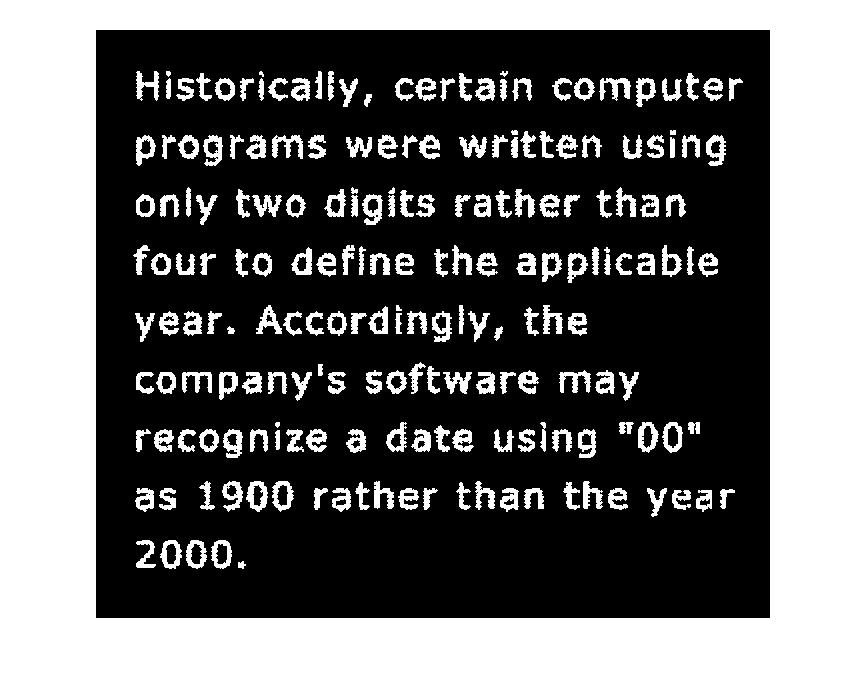
\includegraphics[height=1.2in]{figures/exercise_dilation_02.jpg}
        \caption{imdilate}
    \end{subfigure}%
\end{figure}
\end{homeworkProblem}

%----------------------------------------------------------------------------------------

\newpage

%----------------------------------------------------------------------------------------
%	PROBLEM 2
%----------------------------------------------------------------------------------------

% To have just one problem per page, simply put a \clearpage after each problem

\begin{homeworkProblem}
\maketitle
\subsection{The strel function}
\matlabscript{mfiles/exercise_strel}{The strel function}


\newpage

The function \textbf{se = strel(shape, parameters)} constructs structing elements with a\
 variety of shapes and sizes. Shape is a string specifying the desired shape, and parameters\
is a list of parameters that specify information about the shape, such as size.

In the example, \textbf{SE = strel('diamond', r)} creates a diamond-shaped structuring element,\
where r specifies the distance from the structuring element origin to the points of the diamond.

\begin{figure}[h]
\centering
    \begin{subfigure}[t]{0.3\textwidth}
        \centering
        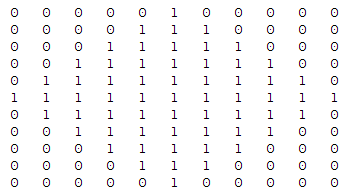
\includegraphics[height=1.2in]{figures/exercise_strel_01.png}
        \caption{r = 5}
    \end{subfigure}%
\end{figure}
\begin{figure}[h]
\centering
    \begin{subfigure}[t]{0.3\textwidth}
        \centering
        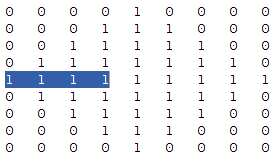
\includegraphics[height=1.2in]{figures/exercise_strel_02.png}
        \caption{r = 4}
    \end{subfigure}%
\end{figure}
\end{homeworkProblem}
%----------------------------------------------------------------------------------------

\newpage

%----------------------------------------------------------------------------------------
%	PROBLEM 3
%----------------------------------------------------------------------------------------

% To have just one problem per page, simply put a \clearpage after each problem

\begin{homeworkProblem}
\maketitle
\subsection{Erosion}
\matlabscript{mfiles/exercise_erosion}{The imerode function}


\newpage

In English, erosion is the process of gradually destroying the surface of something.
The function \textbf{IM2 = imerode(IM,SE)}, erodes the grayscale, binary, or \
packed binary image IM, returning the eroded image IM2. The argument SE is a \
structuring element object or array of structuring element objects returned by \
the strel or offsetstrel functions.

In the block code 1, we want to remove the thin wires in the original image, while \
preserving the other structures. We can do this by choosing a structuring element \
small enough to fit within the center square and thicker border leads but too large \
to git entirely within the wires.

In the block code 2, we choose a structuring element that is too small.

In the block code 3, we choose a stucturing element that is too large. However, I \
cannot get the same result as the text book.
 
\begin{figure}[h]
\centering
    \begin{subfigure}[t]{0.3\textwidth}
        \centering
        
\includegraphics[height=1.2in]{figures/exercise_erosion_01.jpg}
        \caption{Original Image}
    \end{subfigure}%
    \begin{subfigure}[t]{0.3\textwidth}
        \centering
        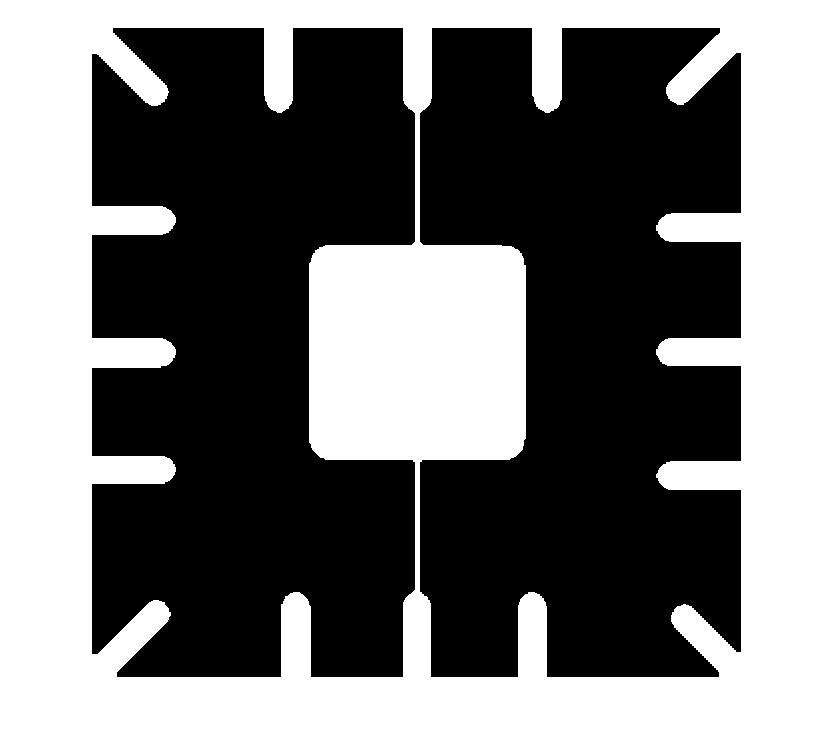
\includegraphics[height=1.2in]{figures/exercise_erosion_02.jpg}
        \caption{r = 10}
    \end{subfigure}%
\end{figure}
\begin{figure}[h]
\centering
    \begin{subfigure}[t]{0.3\textwidth}
        \centering
        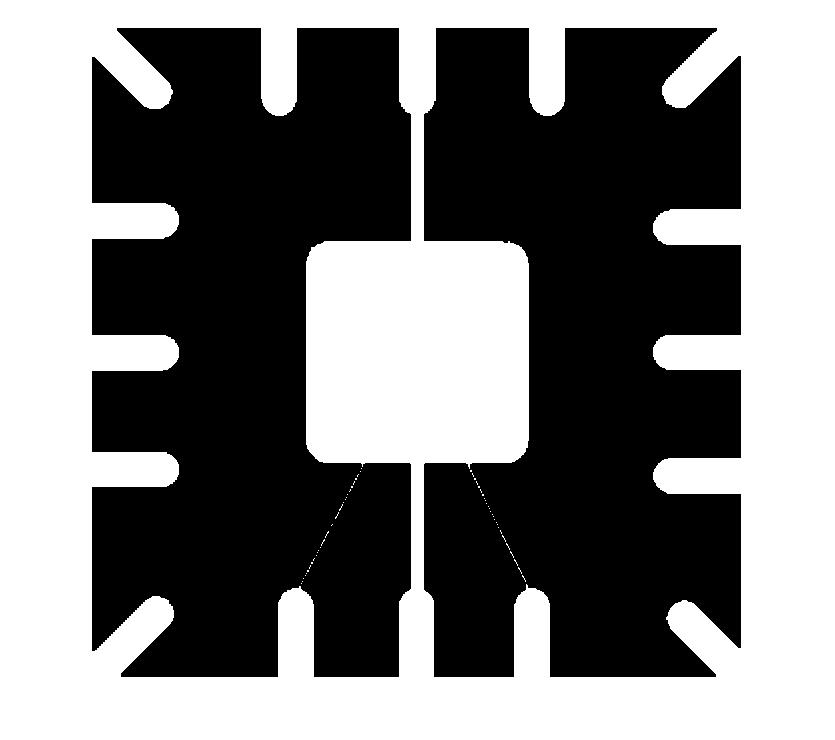
\includegraphics[height=1.2in]{figures/exercise_erosion_03.jpg}
        \caption{r = 5}
    \end{subfigure}%
    \begin{subfigure}[t]{0.3\textwidth}
        \centering
        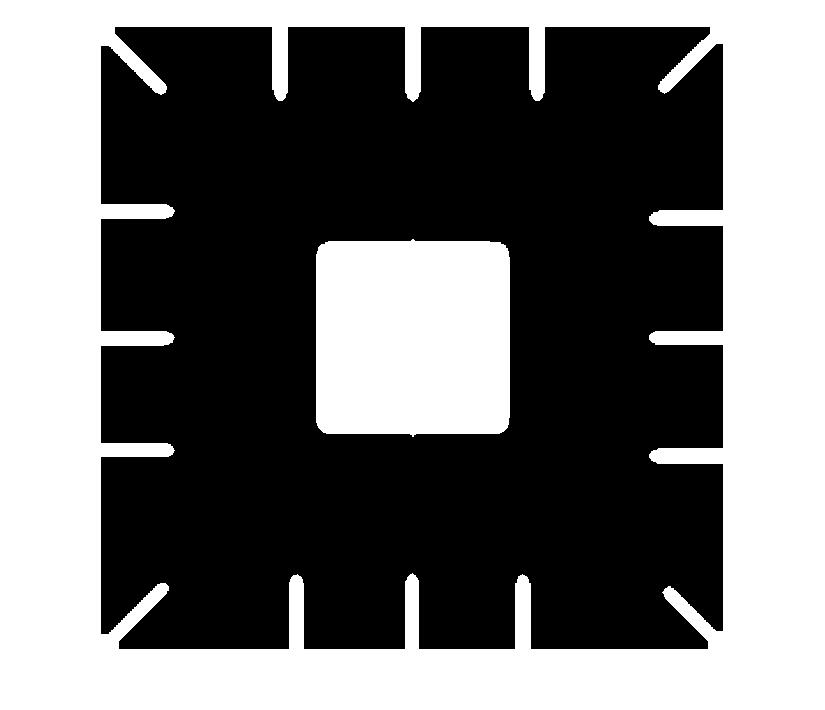
\includegraphics[height=1.2in]{figures/exercise_erosion_04.jpg}
        \caption{r = 20}
    \end{subfigure}%
\end{figure}
\end{homeworkProblem}

%----------------------------------------------------------------------------------------

\newpage

%----------------------------------------------------------------------------------------
%	PROBLEM 4
%----------------------------------------------------------------------------------------

% To have just one problem per page, simply put a \clearpage after each problem

\begin{homeworkProblem}
\maketitle
\subsection{Combining Dilation and Erosion}
\matlabscript{mfiles/exercise_combine_strel_dilation}{Combining Dilation and Erosion}


\newpage

The function \textbf{IM2 = imopen(IM,SE)} performs morphological opening on \
the grayscale or binary image IM with the structuring element SE. The argument \
SE must be a single structuring element object, as opposed to an array of \
objects. The morphological open operation is an erosion followed by a dilation, \
using the same structuring element for both operations.
 
The function \textbf{IM2 = imclose(IM,SE)} performs morphological closing on \
the grayscale or binary image IM, returning the closed image, IM2. The \
structuring element, SE, must be a single structuring element object, as \
opposed to an array of objects. The morphological close operation is a \
dilation followed by an erosion, using the same structuring element for both \
operations.

\begin{figure}[h]
\centering
    \begin{subfigure}[t]{0.3\textwidth}
        \centering
        
\includegraphics[height=1.2in]{figures/exercise_comb_deli_erosion_01.jpg}
        \caption{Original Image}
    \end{subfigure}%
    \begin{subfigure}[t]{0.3\textwidth}
        \centering
        
\includegraphics[height=1.2in]{figures/exercise_comb_deli_erosion_02.jpg}
        \caption{r = 10}
    \end{subfigure}%
\end{figure}
\begin{figure}[h]
\centering
    \begin{subfigure}[t]{0.3\textwidth}
        \centering
        
\includegraphics[height=1.2in]{figures/exercise_comb_deli_erosion_03.jpg}
        \caption{r = 5}
    \end{subfigure}%
\end{figure}

\newpage

An opening/closing sequence can be used for noise reduction.

\begin{figure}[h]
\centering
    \begin{subfigure}[t]{0.3\textwidth}
        \centering
        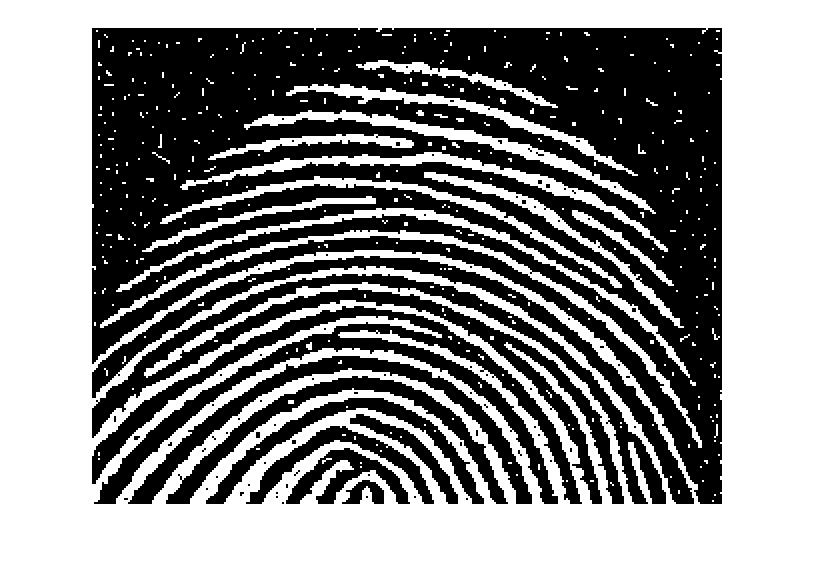
\includegraphics[height=1.2in]{figures/exercise_comb_deli_erosion_04.jpg}
        \caption{Original Image}
    \end{subfigure}%
    \begin{subfigure}[t]{0.3\textwidth}
        \centering
        
\includegraphics[height=1.2in]{figures/exercise_comb_deli_erosion_05.jpg}
        \caption{The noisy spots were removed by opening the image}
    \end{subfigure}%
\end{figure}
\begin{figure}[h]
\centering
    \begin{subfigure}[t]{0.3\textwidth}
        \centering
        
\includegraphics[height=1.2in]{figures/exercise_comb_deli_erosion_06.jpg}
        \caption{final result, in which most of the noise was removed}
    \end{subfigure}%
\end{figure}

\end{homeworkProblem}
%------------------------------------------------------------------------------

%------------------------------------------------------------------------------
%	PROBLEM 5
%------------------------------------------------------------------------------

% To have just one problem per page, simply put a \clearpage after each problem

\begin{homeworkProblem}
\maketitle
\subsection{The Hit-or-Miss Transformation}
\matlabscript{mfiles/exercise_hit_miss}{The Hit-or-Miss Transformation}


\newpage

The function \textbf{BW2 = bwhitmiss(BW1,SE1,SE2)} performs the hit-miss \
operation defined by the structuring elements SE1 and SE2. The hit-miss \
operation preserves pixels whose neighborhoods match the shape of SE1 and \
don't match the shape of SE2. SE1 and SE2 can be flat structuring element \
objects, created by strel, or neighborhood arrays. The neighborhoods of SE1 \
and SE2 should not have any overlapping elements. The syntax \
\textbf{bwhitmiss(BW1,SE1,SE2)} is equivalent to \textbf{imerode(BW1,SE1)} and \
\textbf{imerode(~BW1,SE2)}.

\begin{figure}[h]
\centering
    \begin{subfigure}[t]{0.3\textwidth}
        \centering
        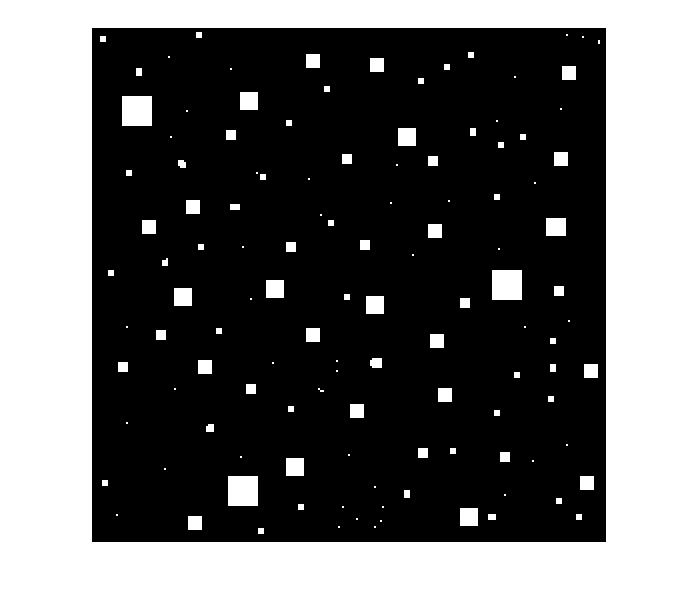
\includegraphics[height=1.2in]{figures/exercise_hit_miss_01.jpg}
        \caption{Original Image}
    \end{subfigure}%
    \begin{subfigure}[t]{0.3\textwidth}
        \centering
        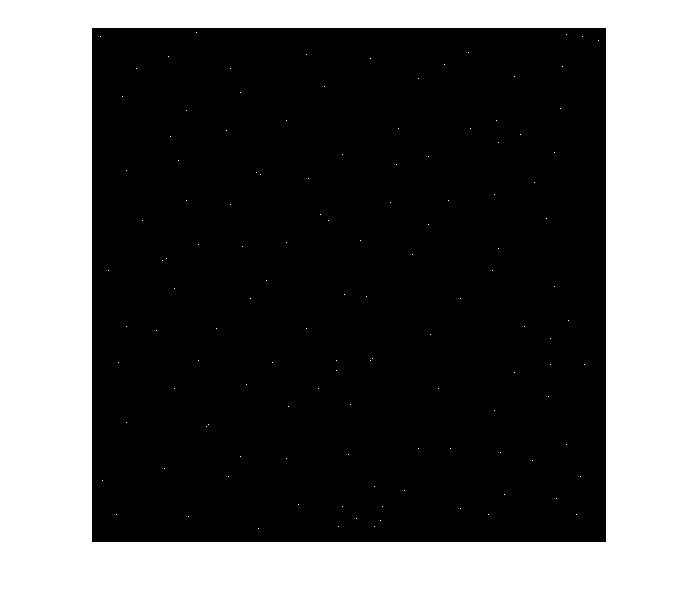
\includegraphics[height=1.2in]{figures/exercise_hit_miss_02.jpg}
        \caption{Result of applying the hitor-miss transformation}
    \end{subfigure}%
\end{figure}
\begin{figure}[h]
\centering
    \begin{subfigure}[t]{0.3\textwidth}
        \centering
        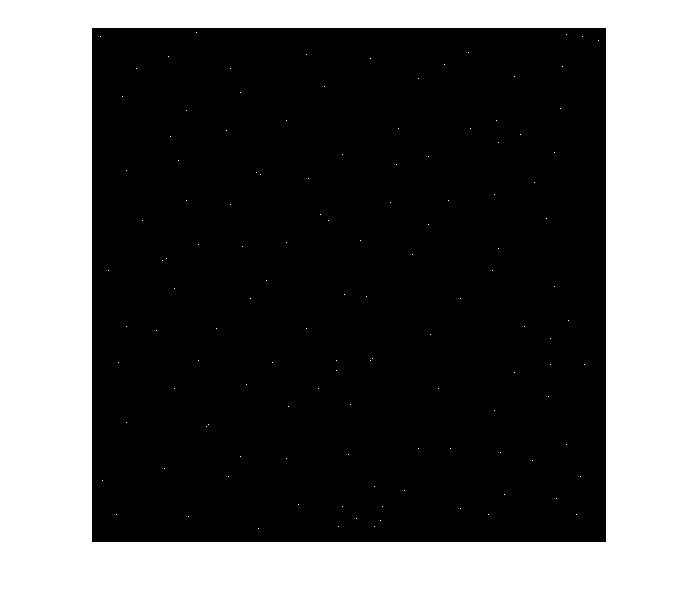
\includegraphics[height=1.2in]{figures/exercise_hit_miss_03.jpg}
        \caption{interval=[ -1 -1 -1; -1 1 1; -1 1 0]}
    \end{subfigure}%
\end{figure}

\newpage

The M-Function \textbf{endpoints} uses \textbf{makelut} and \textbf{applylut} \
to detect end points in a binary image. We define an end point as a foreground \
pixel whose neighbor configuration matches the hit-or-miss interval matrix \
[0 1 0; -1 1 -1; -1 -1 -1] or any of its 90-degree rotations; or a foreground \
pixel whose neighbor configuration matches the hit-or-miss interval matrix \
[1 -1 -1; -1 1 -1; -1 -1 -1] or any of its 90-degree rotations. \
Function \textbf{endpoints} computes and then applies a lookup table for \
detecting end points in an input image.


\begin{figure}[h]
\centering
    \begin{subfigure}[t]{0.3\textwidth}
        \centering
        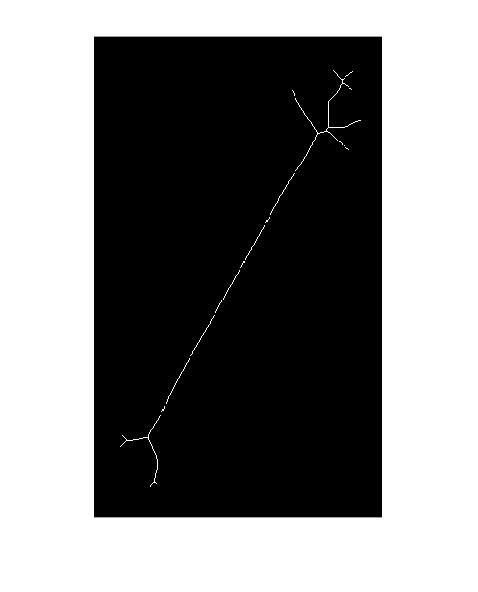
\includegraphics[height=1.2in]{figures/exercise_hit_miss_07.jpg}
        \caption{Original Image}
    \end{subfigure}%
    \begin{subfigure}[t]{0.3\textwidth}
        \centering
        
\includegraphics[height=1.2in]{figures/exercise_hit_miss_08.jpg}
        \caption{Result of applying the hitor-miss transformation}
    \end{subfigure}%
\end{figure}

\newpage

The lookup table is constructed next by calling \textbf{makelut} with a \
function handle to \textbf{conwaylaws}.

\begin{figure}[h]
\centering
    \begin{subfigure}[t]{0.3\textwidth}
        \centering
        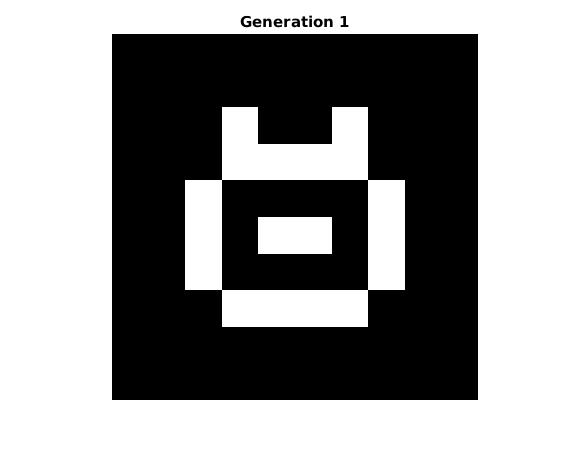
\includegraphics[height=1.2in]{figures/exercise_hit_miss_04.jpg}
        \caption{Original Image}
    \end{subfigure}%
    \begin{subfigure}[t]{0.3\textwidth}
        \centering
        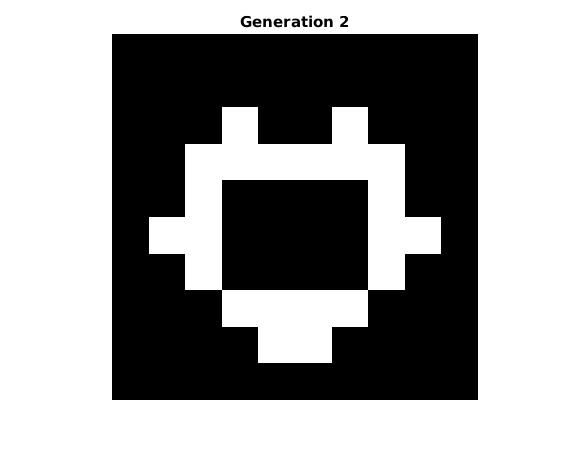
\includegraphics[height=1.2in]{figures/exercise_hit_miss_05.jpg}
        \caption{Generation 2}
    \end{subfigure}%
\end{figure}
\begin{figure}[h]
\centering
    \begin{subfigure}[t]{0.3\textwidth}
        \centering
        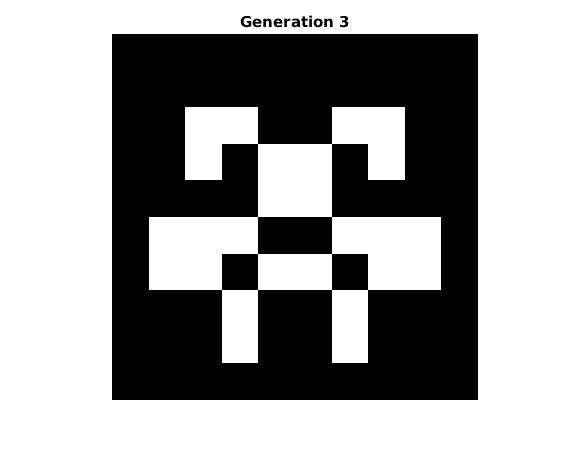
\includegraphics[height=1.2in]{figures/exercise_hit_miss_06.jpg}
        \caption{Generation 3}
    \end{subfigure}%
\end{figure}

\end{homeworkProblem}
%------------------------------------------------------------------------------

%------------------------------------------------------------------------------
%	PROBLEM 6 
%------------------------------------------------------------------------------

% To have just one problem per page, simply put a \clearpage after each problem

\begin{homeworkProblem}
\maketitle
\subsection{Function bwmorph}
\matlabscript{mfiles/exercise_bwmorph}{Function bwmorph}


\newpage
The function \textbf{BW2 = bwmorph(BW,operation)} applies a specific \
morphological operation to the binary image BW.

The function \textbf{bwmorph} implements a variety of morphological operations \
based on combinations of dilations, erosions, and lookup table operations.
\textbf{f} is an input binary image, \textbf{operation} is a string specifying \
the desired operation, and \textbf{n} is a positive integer specifying the \
number of times the operation should be repeated. If argument \textbf{n} \
is omitted, the operation is performed once.

In the textbook, we focus on two operation are: \textbf{thinning} \
and \textbf{skeletonizing}.

If \textbf{n = Inf}, the \textbf{bwmorph} function repeat the operation until \
the image stops changing. This is called repeating an operation\
 \textbf{until stability}.

\textbf{Skeletonization} is a way to reduce binary image objects to a set of \
thin strokes that retain important information about the shape of the original \
object. The skeleton means the main structure that supports a building.

\begin{figure}[h]
\centering
    \begin{subfigure}[t]{0.3\textwidth}
        \centering
        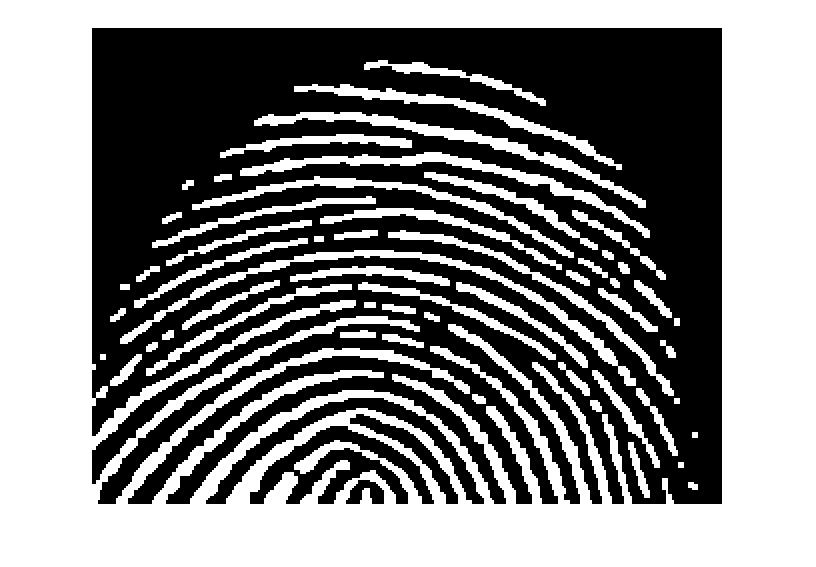
\includegraphics[height=1.2in]{figures/exercise_bwmorph_01.jpg}
        \caption{Original Image}
    \end{subfigure}%
    \begin{subfigure}[t]{0.3\textwidth}
        \centering
        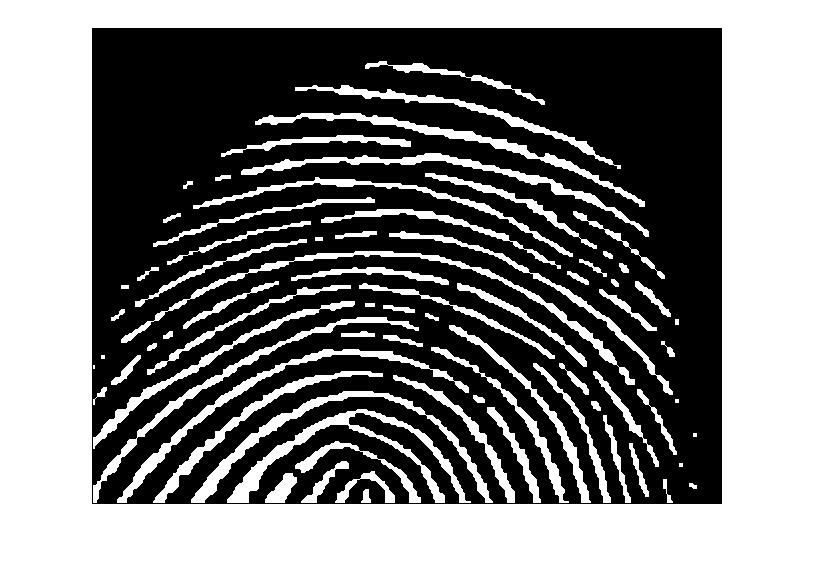
\includegraphics[height=1.2in]{figures/exercise_bwmorph_02.jpg}
        \caption{bwmorph (f, 'thin', 1)}
    \end{subfigure}%
\end{figure}
\begin{figure}[h]
\centering
    \begin{subfigure}[t]{0.3\textwidth}
        \centering
        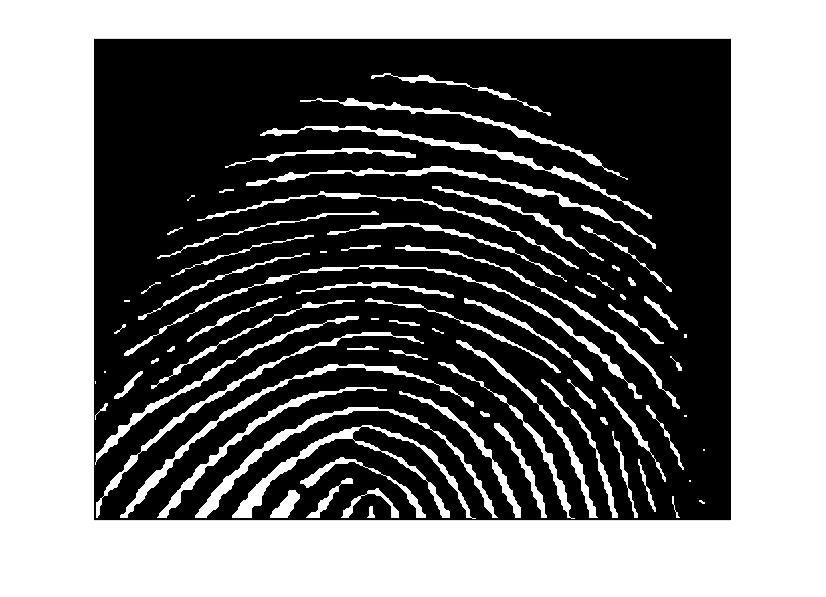
\includegraphics[height=1.2in]{figures/exercise_bwmorph_03.jpg}
        \caption{bwmorph (f, 'thin', 2)}
    \end{subfigure}%
    \begin{subfigure}[t]{0.3\textwidth}
        \centering
        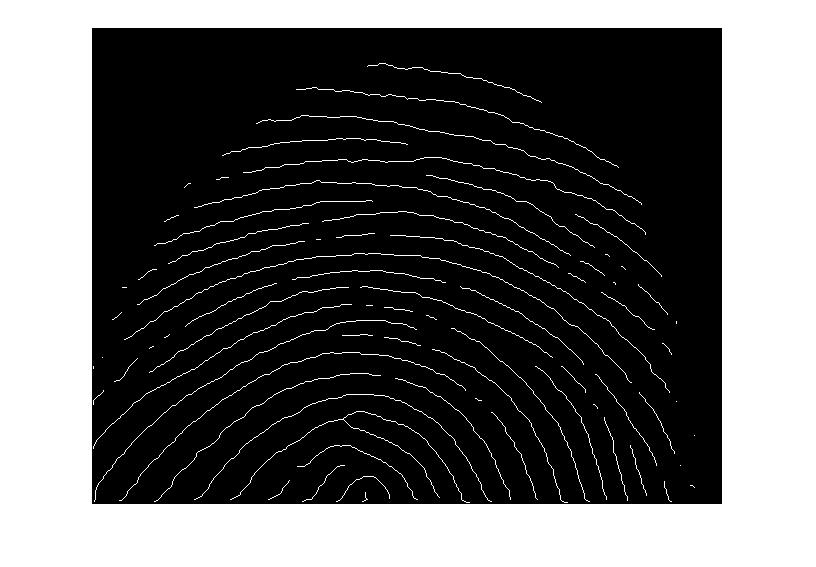
\includegraphics[height=1.2in]{figures/exercise_bwmorph_04.jpg}
        \caption{bwmorph (f, 'thin', 1)}
    \end{subfigure}%
\end{figure}

\begin{figure}[h]
\centering
    \begin{subfigure}[t]{0.3\textwidth}
        \centering
        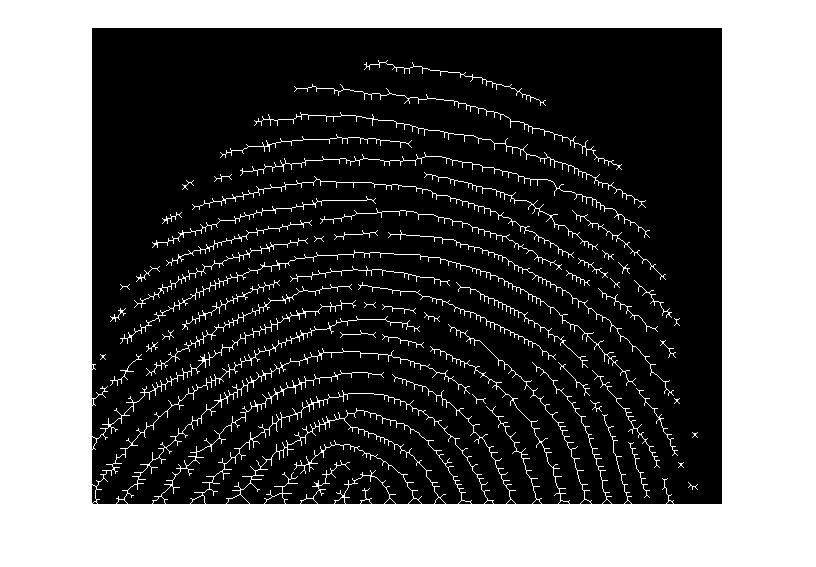
\includegraphics[height=1.2in]{figures/exercise_bwmorph_05.jpg}
        \caption{bwmorph(f, 'skel', Inf)}
    \end{subfigure}%
\end{figure}

\newpage

Skeletonization and thinning often produce short extraneous spurs, called \
parasitic components. The process of cleaning up (or removing) these spurs is
called pruning. We can use function\
 \textbf{fs=bwmorph(fs, 'spur', 5)} for this purpose.

\begin{figure}[h]
\centering
    \begin{subfigure}[t]{0.3\textwidth}
        \centering
        
\includegraphics[height=1.2in]{figures/exercise_bwmorph_07.jpg}
        \caption{Original Image}
    \end{subfigure}%
    \begin{subfigure}[t]{0.3\textwidth}
        \centering
        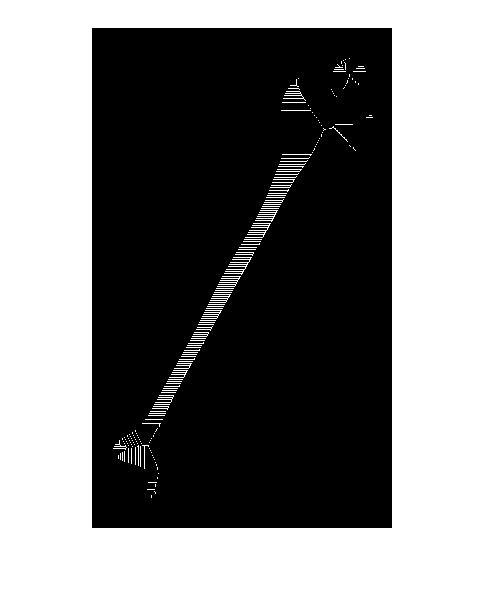
\includegraphics[height=1.2in]{figures/exercise_bwmorph_06.jpg}
        \caption{bwmorph(f, 'skel', Inf)}
    \end{subfigure}%
\end{figure}

\begin{figure}[h]
\centering
    \begin{subfigure}[t]{0.3\textwidth}
        \centering
        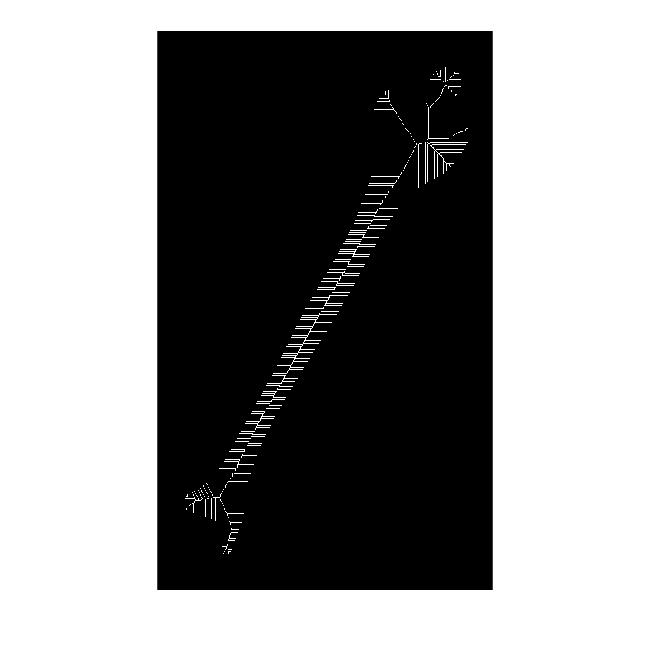
\includegraphics[height=1.2in]{figures/exercise_bwmorph_08.jpg}
        \caption{bwmorph(fs , 'spur', 5)}
    \end{subfigure}%
\end{figure}

\end{homeworkProblem}
%------------------------------------------------------------------------------

\newpage

%------------------------------------------------------------------------------
%	PROBLEM 6 
%------------------------------------------------------------------------------

% To have just one problem per page, simply put a \clearpage after each problem

\begin{homeworkProblem}
\maketitle
\subsection{Reconstruction}
\matlabscript{mfiles/exercise_reconstruction}{Reconstruction}

\newpage

\textbf{IM = imreconstruct(marker,mask)} performs morphological reconstruction \
of the image marker under the image mask. marker and mask can be two intensity \
images or two binary images with the same size. The returned image IM is an \
intensity image or a binary image, depending on the input images, and is \
the same size as the input images.
\textbf{marker} must be the same size as mask, and its elements must be less \
than or equal to the corresponding elements of mask. If the values in marker \
are greater than corresponding elements in mask, imreconstruct clips the \
values to the mask level before starting the procedure.

\begin{figure}[h]
\centering
    \begin{subfigure}[t]{0.3\textwidth}
        \centering
        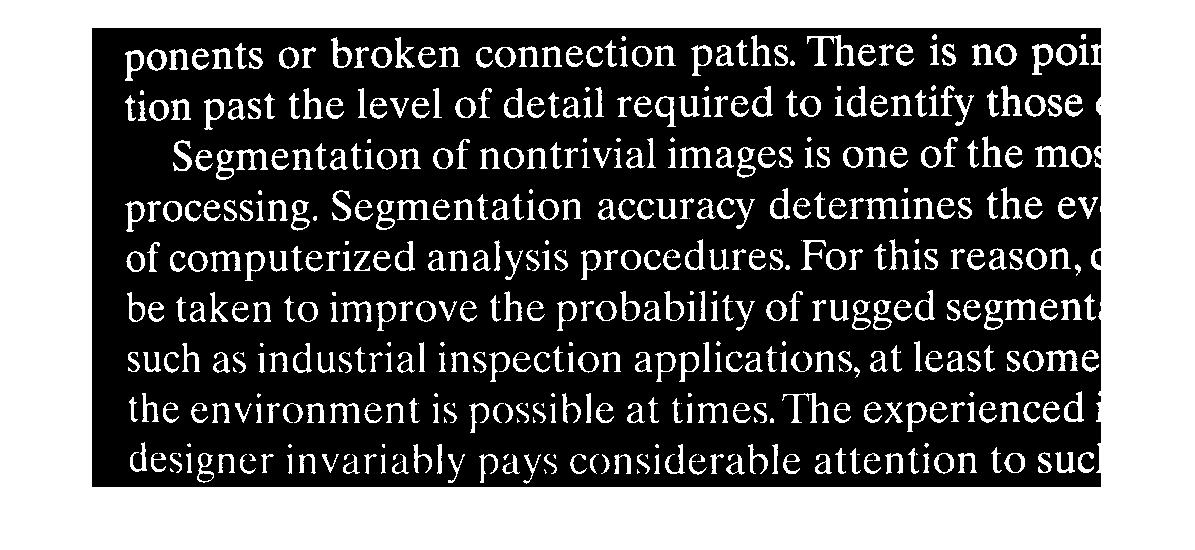
\includegraphics[height=1.2in]{figures/exercise_imreconstruct_01.jpg}
        \caption{Original Image}
    \end{subfigure}%
    \begin{subfigure}[t]{0.3\textwidth}
        \centering
        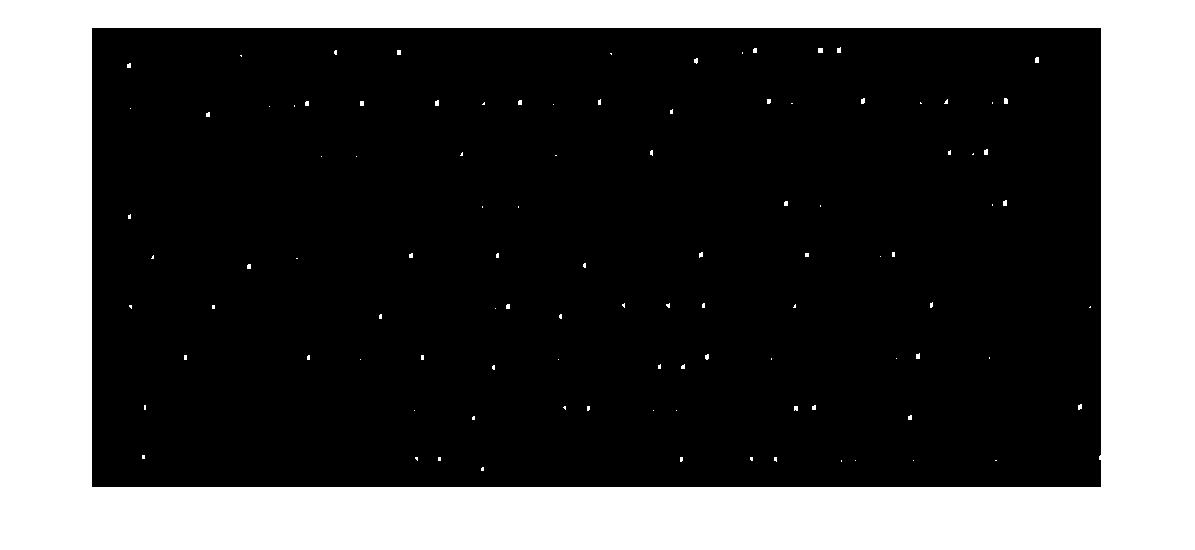
\includegraphics[height=1.2in]{figures/exercise_imreconstruct_02.jpg}
        \caption{imerode(f, ones(51, 1))}
    \end{subfigure}%
\end{figure}
\begin{figure}[h]
\centering
    \begin{subfigure}[t]{0.3\textwidth}
        \centering
        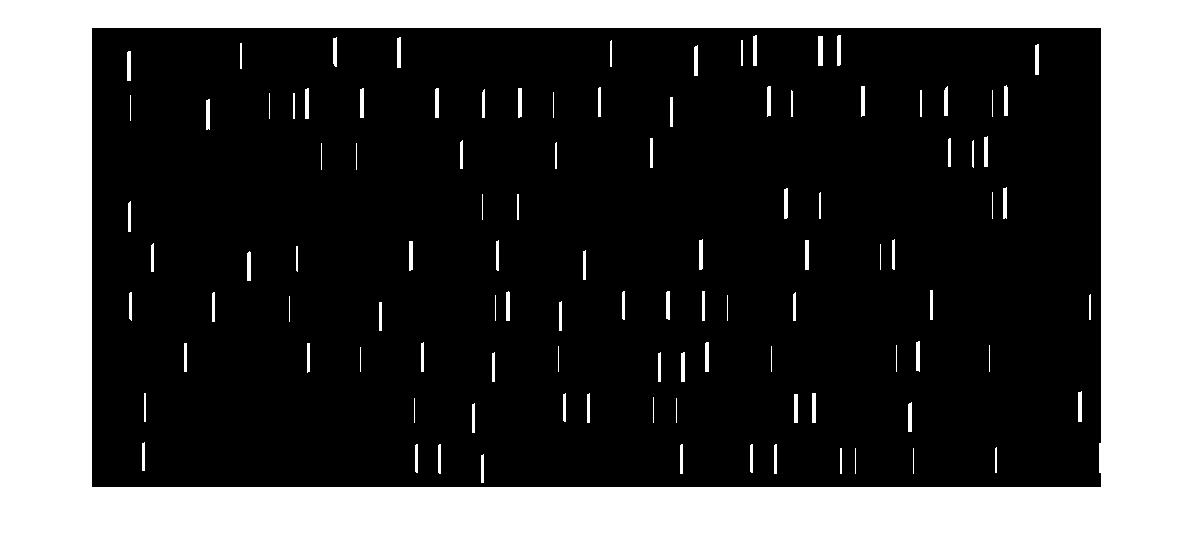
\includegraphics[height=1.2in]{figures/exercise_imreconstruct_03.jpg}
        \caption{imopen(f, ones(51, 1))}
    \end{subfigure}%
    \begin{subfigure}[t]{0.3\textwidth}
        \centering
        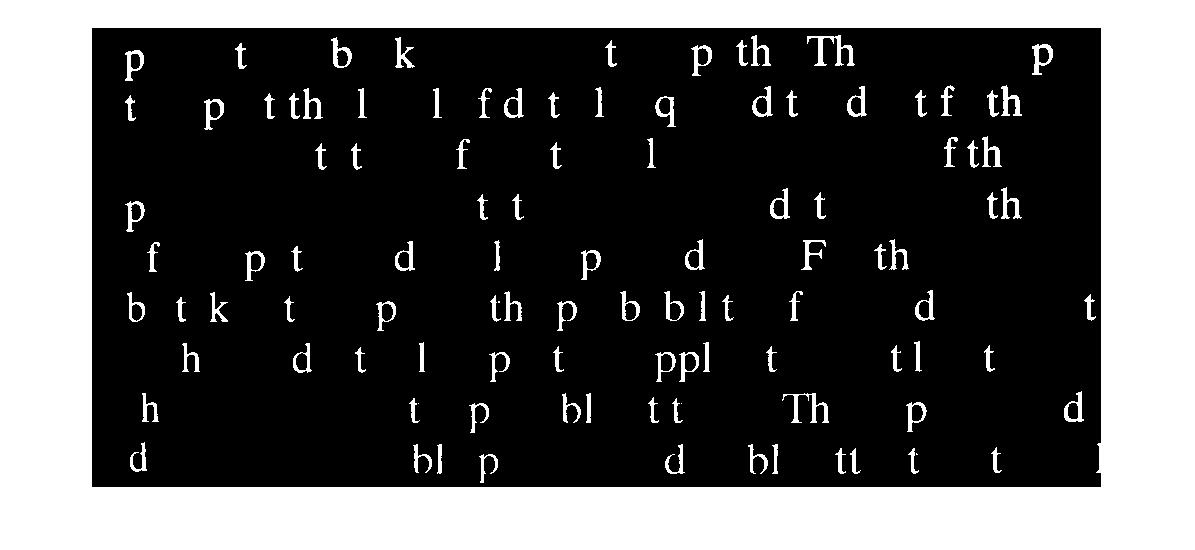
\includegraphics[height=1.2in]{figures/exercise_imreconstruct_04.jpg}
        \caption{imreconstruct(fe, f)}
    \end{subfigure}%
\end{figure}

\end{homeworkProblem}
%------------------------------------------------------------------------------

\end{document}
